\documentclass[10pt]{article}
\usepackage[a4paper,margin=0.72in]{geometry}
\usepackage[T1]{fontenc}
\usepackage[utf8]{inputenc}
\usepackage{lmodern}
\usepackage[numbers,sort&compress]{natbib}
\usepackage{graphicx}
\usepackage{booktabs}
\usepackage{amsmath}
\usepackage{enumitem}
\usepackage{caption}
\usepackage{float}
\usepackage[colorlinks=true,linkcolor=blue,citecolor=blue,urlcolor=blue]{hyperref}

\setlength{\parindent}{0pt}
\setlength{\parskip}{0.34em}
\setlist{nosep,leftmargin=1.4em}
\captionsetup{font=small}

\title{\vspace{-1.2em}\textbf{Game Playing with Reinforcement Learning on Stochastic FrozenLake}\\[-0.25em]
{\large Benchmarking Tabular Agents on Standard and Controlled Maps}}
\author{Group 8: Chi Kit WONG, Haodong XU, Sida ZHANG\\
AIAA3053 Reinforcement Learning Principles and Methods}
\date{}

\begin{document}
\maketitle
\vspace{-1.8em}

\begin{abstract}
This project studies FrozenLake as a stochastic grid-world game-playing task. A player-controlled agent starts from the start tile, avoids holes, and tries to reach the goal; in the slippery version, the executed move may deviate from the intended move. We therefore treat the problem as game playing under transition uncertainty rather than deterministic maze solving. Starting from an initial 4$\times$4 Q-learning implementation, we build a broader RL game-agent comparison across Q-learning, SARSA, Expected SARSA, SARSA($\lambda$), Q($\lambda$), Dyna-Q, and optimistic Q-learning, with Value Iteration as a known-model oracle. A central part of the project is the evolution of the experimental design. We first used Gymnasium as a reference point: the standard Gymnasium 8$\times$8 map is a strong benchmark and sanity check, while Gymnasium-generated low-$p$ random maps revealed a problem--many are connected but nearly impossible under slippery dynamics. We therefore introduced controlled maps: designed 4$\times$4 maps with exactly four holes and oracle filtering, plus controlled random 8$\times$8 maps with fixed frozen-tile probabilities and guaranteed connectivity. These maps are solvable, non-trivial, reproducible, and better suited for comparing game-playing agents. On the controlled random 8$\times$8 benchmark, optimistic Q-learning reaches 0.988 mean final success, followed by Expected SARSA and SARSA above 0.89. The Gymnasium standard 8$\times$8 result is retained as an important standard game benchmark, and the Gymnasium random-map results are retained as a diagnostic motivation for careful map design.
\end{abstract}

\section{Introduction}
FrozenLake is a compact game-playing environment for reinforcement learning (RL). The game board is a frozen grid: the player starts at \texttt{S}, tries to reach \texttt{G}, and loses the episode by falling into a hole \texttt{H}. Rewards are sparse: the agent receives reward 1 only at the goal and 0 elsewhere. In the slippery version, an intended move can slip to a neighboring direction, so the task is not simply finding a shortest path. A good game-playing policy must choose actions that remain robust when the environment executes a nearby unintended move.

The original course project theme was game playing with Q-learning. The initial implementation already trained a Q-learning agent on 4$\times$4 FrozenLake, but it left three open questions: whether other RL game-playing agents behave differently, whether results hold beyond a single small board, and whether hyperparameter choices are credible. This report addresses those questions with a stochastic-only benchmark, controlled map design, and focused ablation studies. The final benchmark was not chosen blindly: it was shaped by the contrast between the useful Gymnasium standard 8$\times$8 game board and the often near-impossible Gymnasium low-$p$ random boards.

The research questions are:
\begin{enumerate}
    \item Which tabular RL game-playing agents are strongest on slippery FrozenLake?
    \item Why is controlled board design necessary for fair algorithm comparison on stochastic FrozenLake?
    \item Is performance mainly limited by exploration or reward propagation?
    \item Does automated hyperparameter search improve the strongest methods?
\end{enumerate}

\section{Related Work}
Q-learning is a classical off-policy temporal-difference control method that uses a max next-state target \cite{WatkinsDayan1992}. SARSA and Expected SARSA are on-policy alternatives that update values under the behavior policy rather than an ideal greedy target \cite{SuttonBarto2018}. Eligibility-trace methods such as SARSA($\lambda$) and Q($\lambda$) propagate TD errors through recent state-action trajectories, which can help sparse rewards reach earlier decisions \cite{SuttonBarto2018}. Dyna-Q combines model-free learning with planning updates from a learned transition model, reusing scarce experience more efficiently \cite{SuttonBarto2018}. Double Q-learning reduces overestimation bias in noisy value estimates \cite{VanHasselt2010}, though this conservatism can slow discovery when rewards are rare.

FrozenLake is widely used in Gymnasium teaching material for Q-learning and map-size sensitivity \cite{GymnasiumFrozenLakeTutorial}. Our study follows the same qualitative motivation but adds a broader tabular comparison, oracle references, Optuna tuning, and controlled random-map tests. For tuning, we use Optuna's Tree-structured Parzen Estimator (TPE) sampler \cite{OptunaTPESampler}. Larger distributed sweeps could use Ray Tune with ASHA/HyperBand \cite{RayTuneSchedulers}, but Optuna is lightweight and appropriate for the current coursework-scale experiments.

\section{Methodology}
\subsection{Experimental Design Evolution}
The experiment was developed in three stages. First, we used the standard FrozenLake boards as references. The standard 4$\times$4 board keeps the project close to the original Q-learning implementation, while the standard Gymnasium 8$\times$8 board is valuable because it is widely recognized, reproducible, and neither trivial nor impossible under \texttt{slippery=True}. These two boards serve as sanity checks for the training and evaluation pipeline.

Second, we moved from the standard Gymnasium board to library-generated random boards. Gymnasium's random-map generator guarantees that a path exists from start to goal, but in slippery FrozenLake deterministic reachability is not enough. A board can contain a valid path while still having very low optimal success probability, because slips can repeatedly push the agent into holes. In our Gymnasium random-map trial, many $p=0.5$ and $p=0.6$ boards produced near-zero oracle success and near-zero learned success for every algorithm. Such boards are useful as stress tests, but they are not useful for ranking algorithms because the dominant factor is board impossibility rather than learning quality.

Third, we introduced controlled maps for the final comparison. The design goal is not to make the problem easy, but to make it comparable: each board should be stochastic, solvable, non-trivial, and reproducible. We therefore keep the standard boards for baseline comparability, use Gymnasium-generated random boards as a diagnostic failure case, and use controlled 4$\times$4 and 8$\times$8 boards for the main algorithm comparison.

\subsection{FrozenLake Game Environment}
All reported experiments use \texttt{slippery=True}. In each step, the environment samples one of three outcomes: the intended direction, the left deviation, or the right deviation, each with probability $1/3$. This matches the standard FrozenLake stochastic transition idea and prevents the task from becoming deterministic maze following.

We evaluate six stochastic settings:
\begin{itemize}
    \item \textbf{Standard 4x4}: the Gym-style map \texttt{SFFF/FHFH/FFFH/HFFG}, with four holes out of sixteen cells.
    \item \textbf{Gymnasium standard 8x8}: the library standard 8x8 map, used as a key standard comparison and sanity check.
    \item \textbf{Gymnasium random-map diagnostic}: generated Gymnasium maps at $p\in\{0.8,0.7,0.6,0.5\}$, three maps per $p$. This trial motivated controlled-map design because many low-$p$ maps had near-zero oracle success.
    \item \textbf{Designed 4x4}: random maps with exactly four holes, BFS reachability checks, and Value Iteration oracle filtering.
    \item \textbf{Fixed 8x8}: the standard fixed 8x8 benchmark map used in the project.
    \item \textbf{Controlled random 8x8}: random maps with $p\in\{0.80,0.85,0.90,0.95\}$, five maps per difficulty. These maps are the main 8x8 algorithm-comparison benchmark.
\end{itemize}

\subsection{Controlled Board Generation}
The controlled boards were generated before algorithm training and were not selected according to learned-agent performance. For the designed 4$\times$4 setting, we sample exactly four hole positions from the 14 non-terminal cells. This matches the hole count of the standard 4$\times$4 board and avoids the earlier problem where high-$p$ random maps accidentally contained too few holes. Each candidate is then checked with a shortest-path BFS from start to goal. Unreachable boards are rejected. Finally, a Value Iteration oracle is evaluated under \texttt{slippery=True}; boards with oracle success below 0.55 are rejected as too hard, and boards above 0.95 are rejected as too easy. The accepted 4$\times$4 boards therefore have the same hole count, deterministic reachability, and a non-degenerate stochastic oracle range.

For the controlled random 8$\times$8 setting, we generate five boards at each frozen-tile probability $p\in\{0.80,0.85,0.90,0.95\}$. A random grid is first sampled with probability $p$ for frozen tiles. Then a safe start-to-goal corridor is carved by moving randomly right or down until the goal is reached. This guarantees deterministic connectivity without making every surrounding tile safe. We then compute and report the Value Iteration oracle for each board. These 8$\times$8 boards are therefore not arbitrary impossible random maps; they are controlled stochastic games with known layouts, known oracle references, and enough map-to-map variation to compare algorithms.

This controlled design prevents two opposite failure modes. Unconstrained high-$p$ random generation can create trivial maps with too few holes, while low-$p$ Gymnasium generation can create connected but almost impossible slippery boards. The controlled maps sit between these extremes, making the final comparison about learning behavior rather than accidental map pathology.

\subsection{RL Game-Playing Agents and Metrics}
The main comparison uses seven learned tabular game-playing agents: Q-learning, SARSA, Expected SARSA, SARSA($\lambda$), Q($\lambda$), Dyna-Q, and optimistic Q-learning. The exploration ablation additionally compares UCB-Q and softmax Q-learning. Value Iteration is used as an oracle, not as a fair model-free competitor, because it uses the known transition model.

The primary game-playing metric is greedy evaluation success rate after training: how often the learned policy reaches the goal before falling into a hole or exceeding the step limit. We also report standard deviation across seeds or maps and compare learned policies against the Value Iteration oracle. A high oracle score with a low learned score means the board is solvable but the learning algorithm failed to discover or propagate reward efficiently.

\section{Results}
\subsection{Standard 4x4 Baseline}
Figure~\ref{fig:standard4} shows the latest standard 4$\times$4 slippery rerun. The oracle reaches 0.847 success, which confirms that the stochastic setting is not expected to reach a guaranteed 1.0 success rate. Q-learning reaches 0.770, optimistic Q-learning reaches 0.767, SARSA reaches 0.723, and Expected SARSA reaches 0.680. These values are plausible for slippery FrozenLake and avoid the misleading 1.0 success rates from overly easy random maps.

\begin{figure}[H]
    \centering
    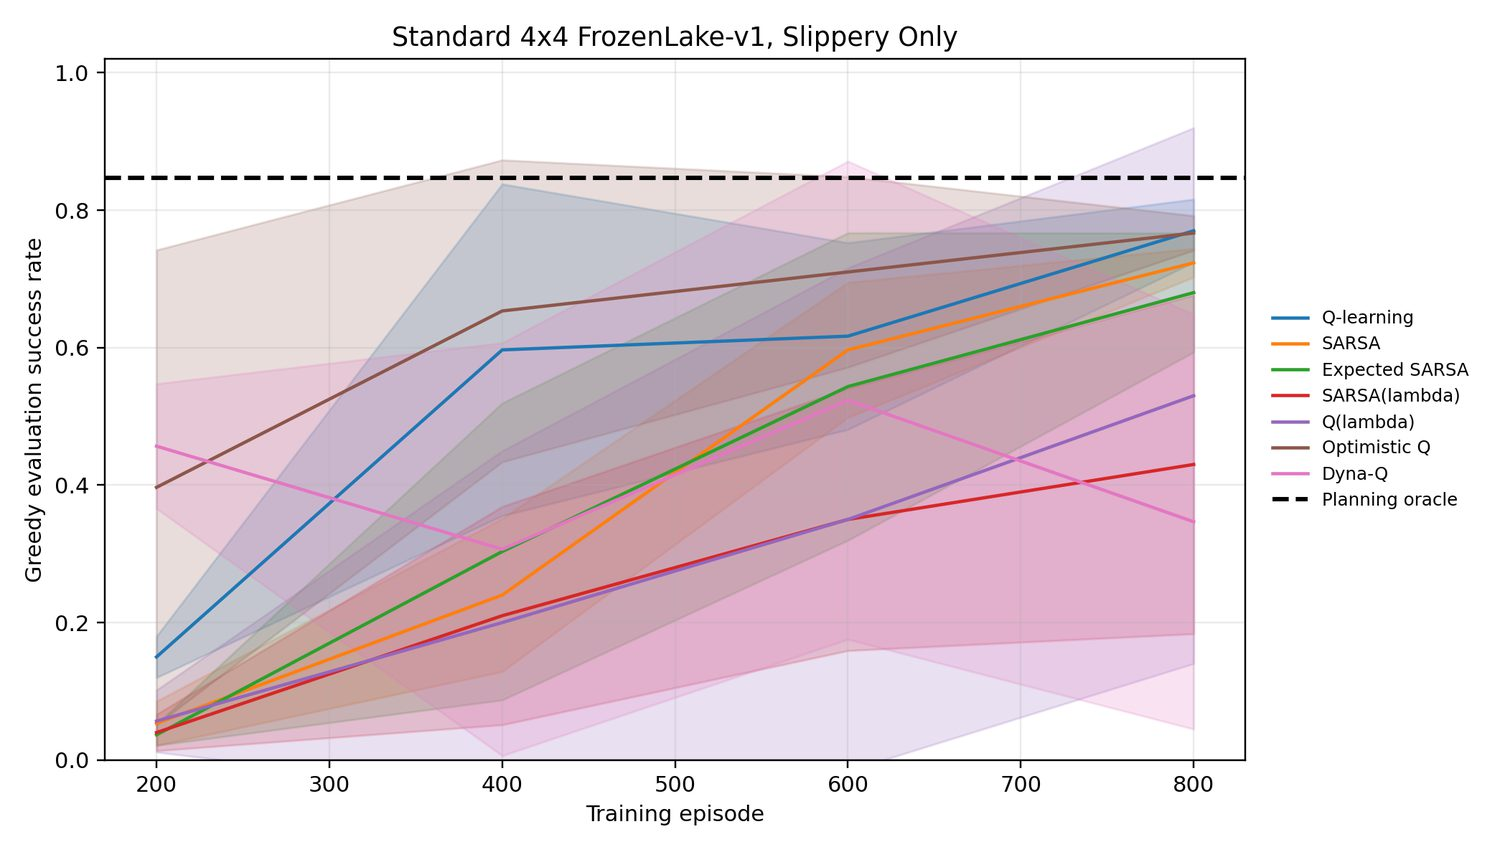
\includegraphics[width=0.78\linewidth]{figures_compact/standard_4x4_slippery_only_success.jpg}
    \caption{Standard 4$\times$4 slippery FrozenLake results. The map has four holes, and all evaluation is stochastic.}
    \label{fig:standard4}
\end{figure}

\subsection{Gymnasium Standard 8x8 and Random-Map Diagnostic}
The next step was to test whether the same pipeline works on Gymnasium's standard 8$\times$8 board and on Gymnasium-generated random boards. This order matters for the story of the project: the controlled maps were introduced after observing the limitations of direct random-map generation.

The standard Gymnasium 8$\times$8 map is an important benchmark. It is widely used, reproducible, and challenging without being degenerate. In our run, its oracle success is 0.861, and the learned mean success across the seven algorithms is 0.709. Several algorithms learn strong policies on this map: Expected SARSA reaches 0.85, Q($\lambda$) reaches 0.85, optimistic Q-learning reaches 0.82, Q-learning reaches 0.78, SARSA($\lambda$) reaches 0.76, and SARSA reaches 0.74. This confirms that the training pipeline can handle a standard stochastic 8$\times$8 benchmark.

Gymnasium-generated random maps answer a different design question: what happens if we rely directly on the library's random-map generator at lower frozen-tile probabilities? The answer is that performance drops sharply on many generated random maps, and the reason is visible from the oracle. Several $p=0.5$ and $p=0.6$ random maps have oracle success near zero under slippery dynamics. These maps are technically connected, because the generator guarantees a path from start to goal, but the stochastic transition model makes reliable completion extremely unlikely. Across all 13 Gymnasium maps, including the standard map and the random maps, optimistic Q-learning remains the best learned method, but its mean final success is only 0.235 because the near-impossible generated maps dominate the average. This diagnostic result explains why the project moved toward carefully controlled maps for fair algorithm ranking.

\begin{figure}[H]
    \centering
    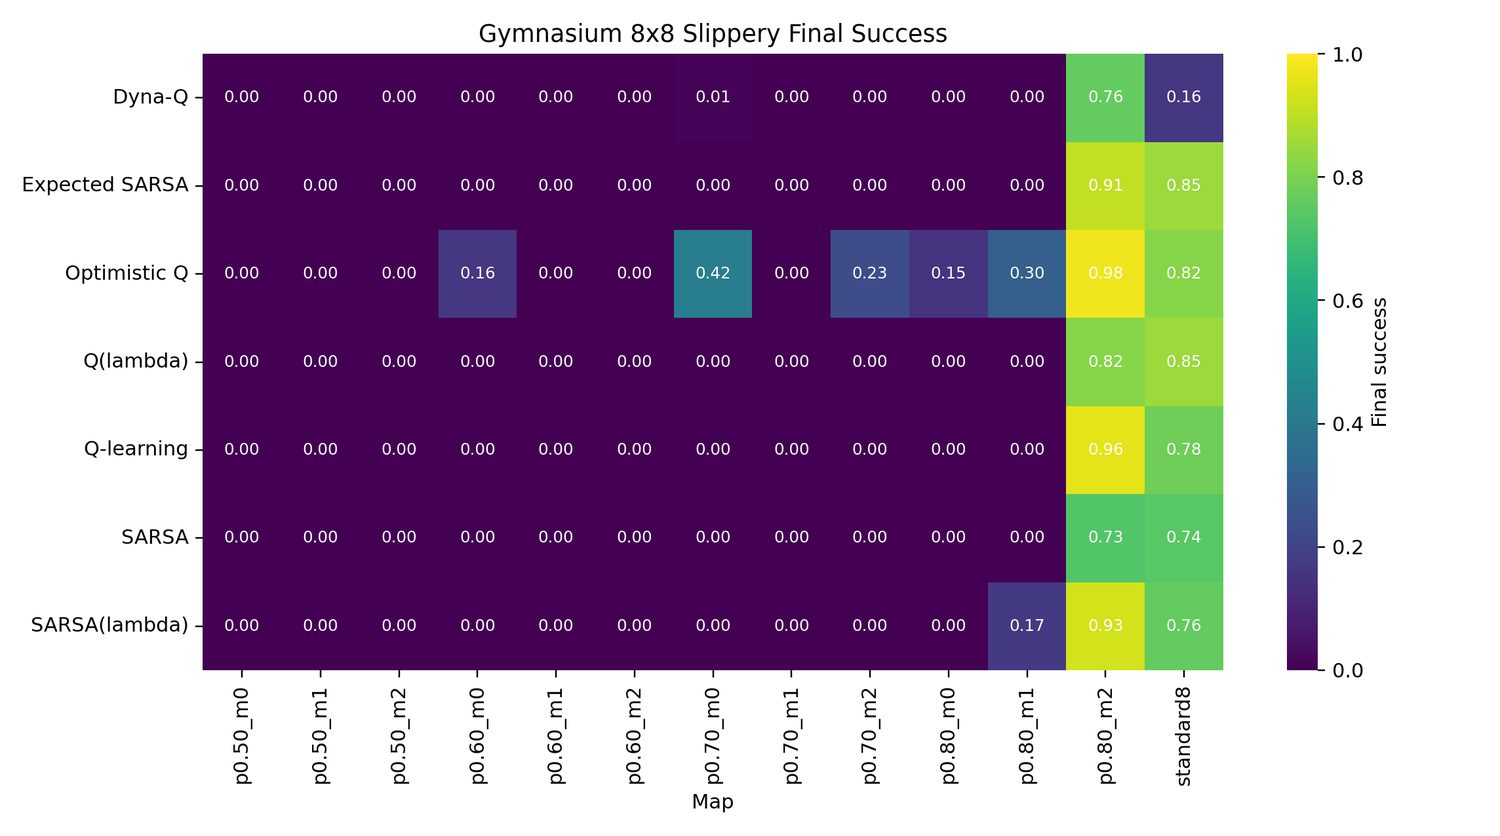
\includegraphics[width=0.96\linewidth]{figures_compact/gymnasium8/gym8_final_success_heatmap.jpg}
    \caption{Gymnasium 8$\times$8 slippery final success. The standard 8$\times$8 map is a useful benchmark, while several low-$p$ generated maps are too difficult for fair ranking.}
    \label{fig:gym8success}
\end{figure}

\begin{figure}[H]
    \centering
    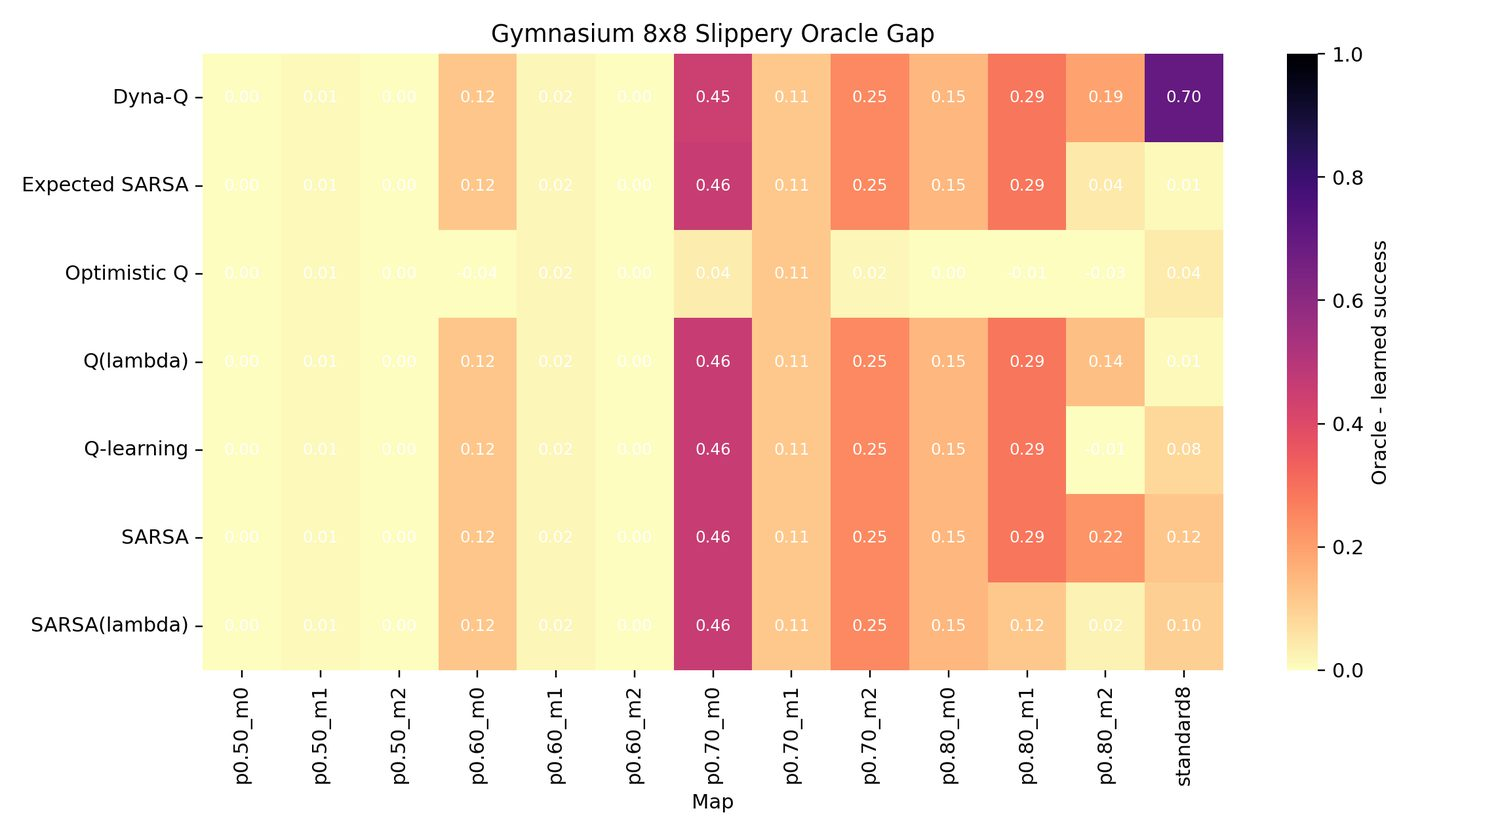
\includegraphics[width=0.96\linewidth]{figures_compact/gymnasium8/gym8_oracle_gap_heatmap.jpg}
    \caption{Oracle gap on Gymnasium 8$\times$8 maps. The standard map is solvable, while several generated low-$p$ maps are almost impossible under slippery dynamics.}
    \label{fig:gym8gap}
\end{figure}

\subsection{Controlled 4x4 Maps}
Figure~\ref{fig:designed4} reports the controlled random 4$\times$4 experiment. These maps also have exactly four holes and are therefore much more credible than high-$p$ random maps. With the longer 2,000-episode learning-curve rerun, Expected SARSA and Q-learning are the strongest mean final-success methods on these four maps, while optimistic Q-learning has the best mean AUC, meaning that it often learns earlier even when the final score is not always the highest.

\begin{figure}[H]
    \centering
    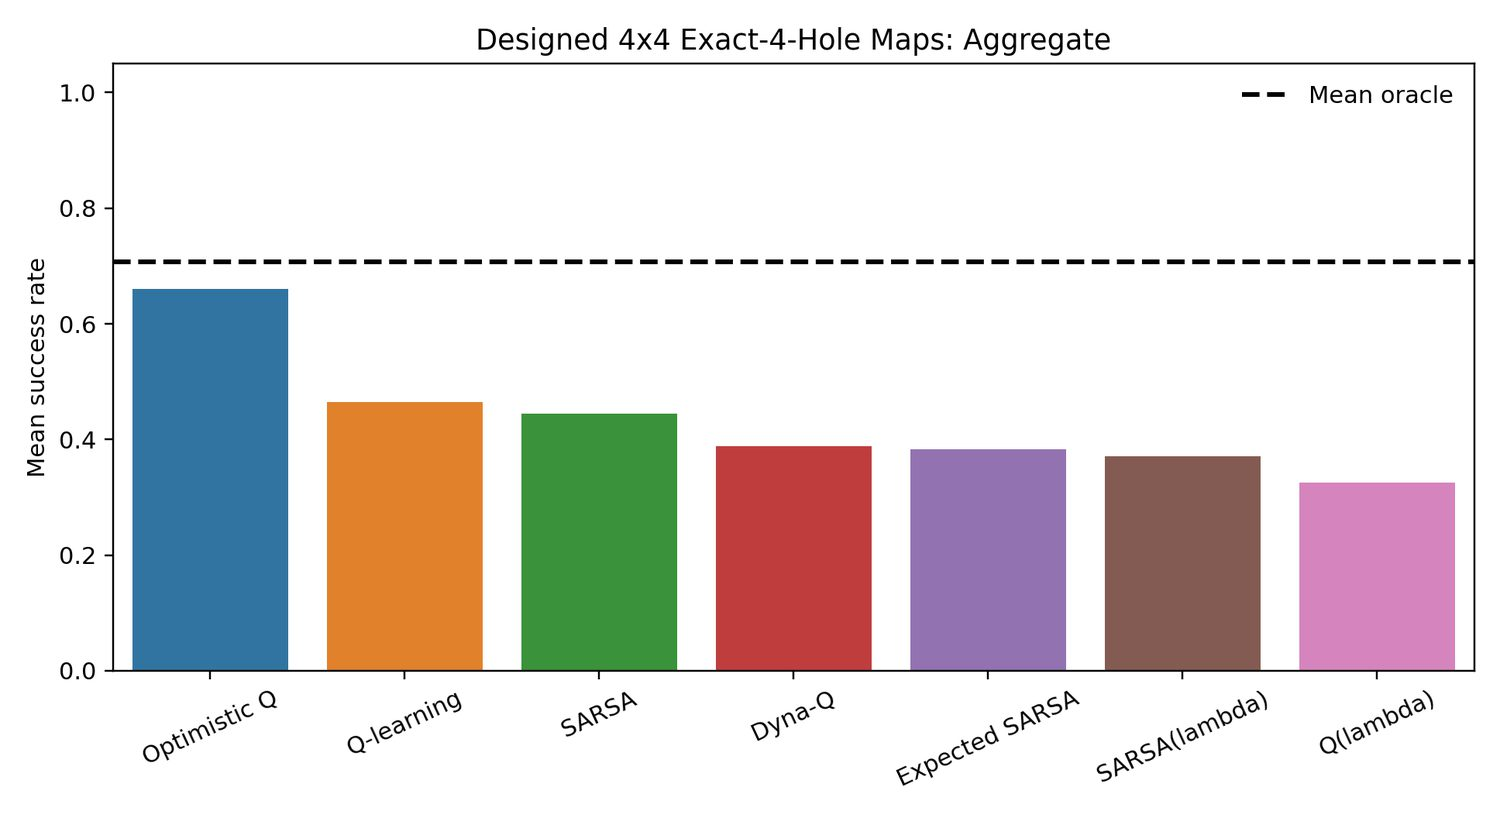
\includegraphics[width=0.82\linewidth]{figures_compact/designed_4x4_exact4holes_aggregate.jpg}
    \caption{Designed random 4$\times$4 maps with exactly four holes. This is the controlled random-map counterpart to the standard 4$\times$4 map.}
    \label{fig:designed4}
\end{figure}

\subsection{Controlled 8x8 Stochastic Benchmark}
The controlled 8$\times$8 setting is the main comparison benchmark in this report. It is more informative than 4$\times$4 because sparse reward is harder to discover and the longer paths expose differences between exploration and reward-propagation strategies. At the same time, the maps are not arbitrary hard instances: they are designed to be solvable under slippery dynamics, so a low score is more likely to reflect the algorithm rather than an almost impossible layout.

Figure~\ref{fig:summaryheatmap} summarizes the updated stochastic results. The random 8$\times$8 numbers use 10,000 training episodes with evaluation every 500 episodes. Optimistic Q-learning is the strongest learned method on controlled random 8$\times$8, reaching 0.988 mean final success over 20 maps. Expected SARSA, SARSA, Q-learning, Q($\lambda$), and Dyna-Q also improve substantially under the longer budget. These are the results that best support an algorithm-comparison story for the presentation and report.

\begin{figure}[H]
    \centering
    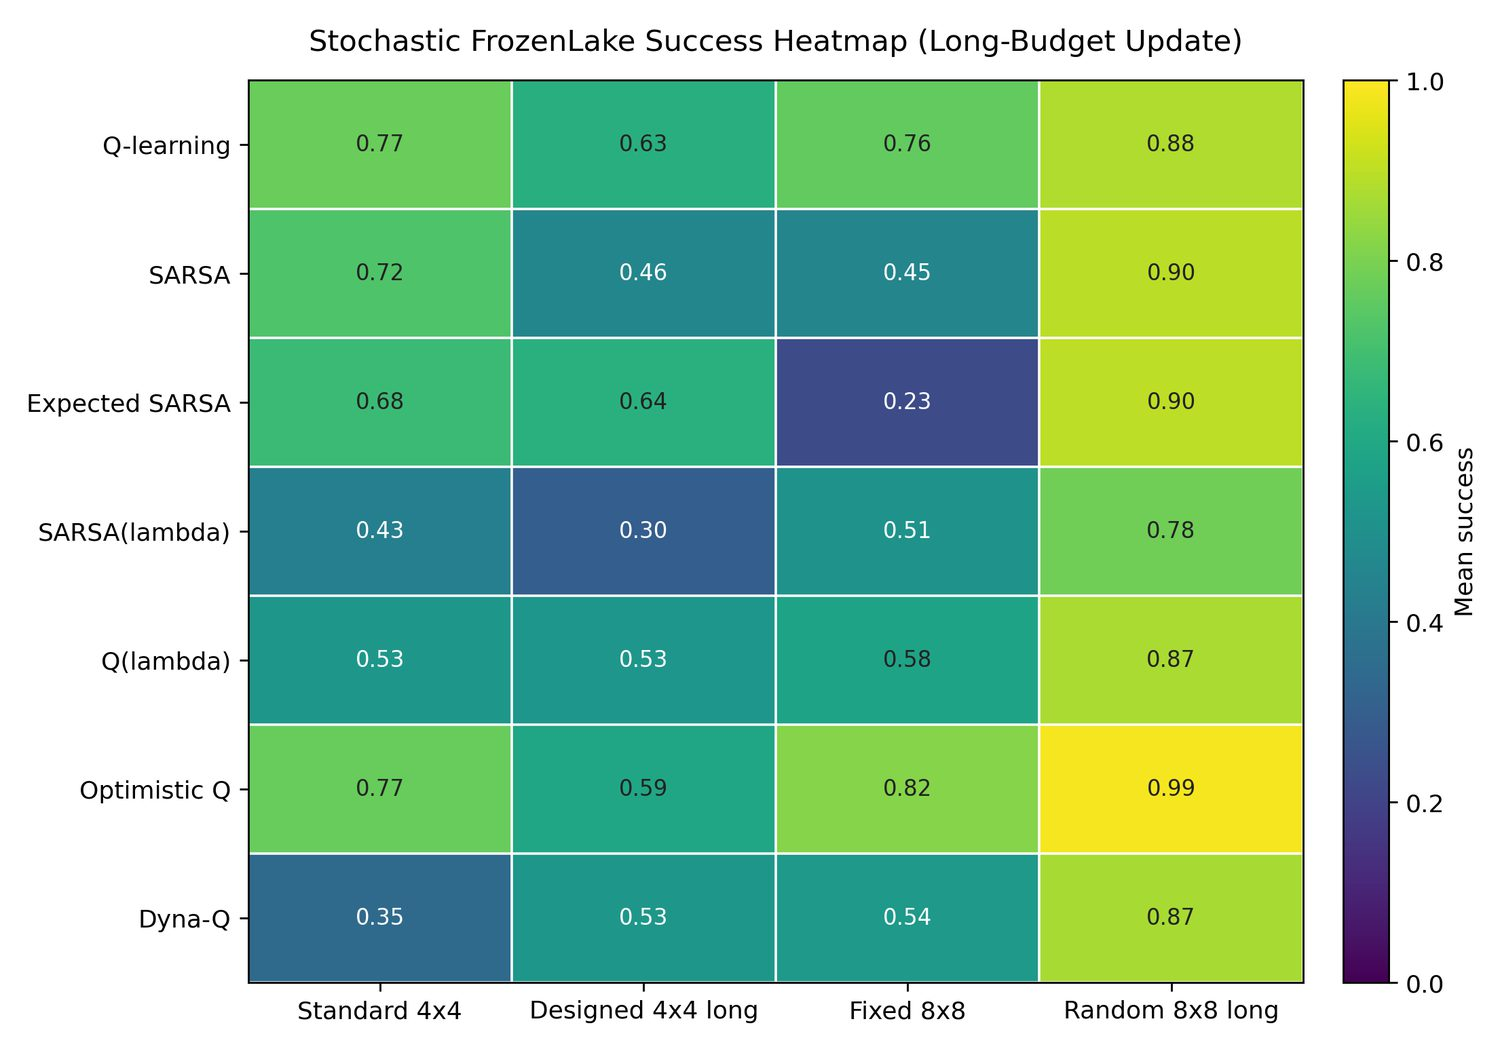
\includegraphics[width=0.92\linewidth]{figures_compact/stochastic_success_heatmap.jpg}
    \caption{Mean success rate across the stochastic benchmark. The heatmap uses explicit per-cell text annotations and includes the long-budget random-map update.}
    \label{fig:summaryheatmap}
\end{figure}

Figure~\ref{fig:difficulty} shows the long-budget controlled random 8$\times$8 difficulty sweep. Each point is an individual map, and the short horizontal marks indicate the mean for each algorithm and frozen-tile probability. This version is more interpretable than a single aggregate line plot because it exposes map-to-map variation directly. The high scores should therefore be interpreted as ``solving the controlled stochastic benchmark'', not as solving every possible randomly generated 8$\times$8 FrozenLake map.

\begin{figure}[H]
    \centering
    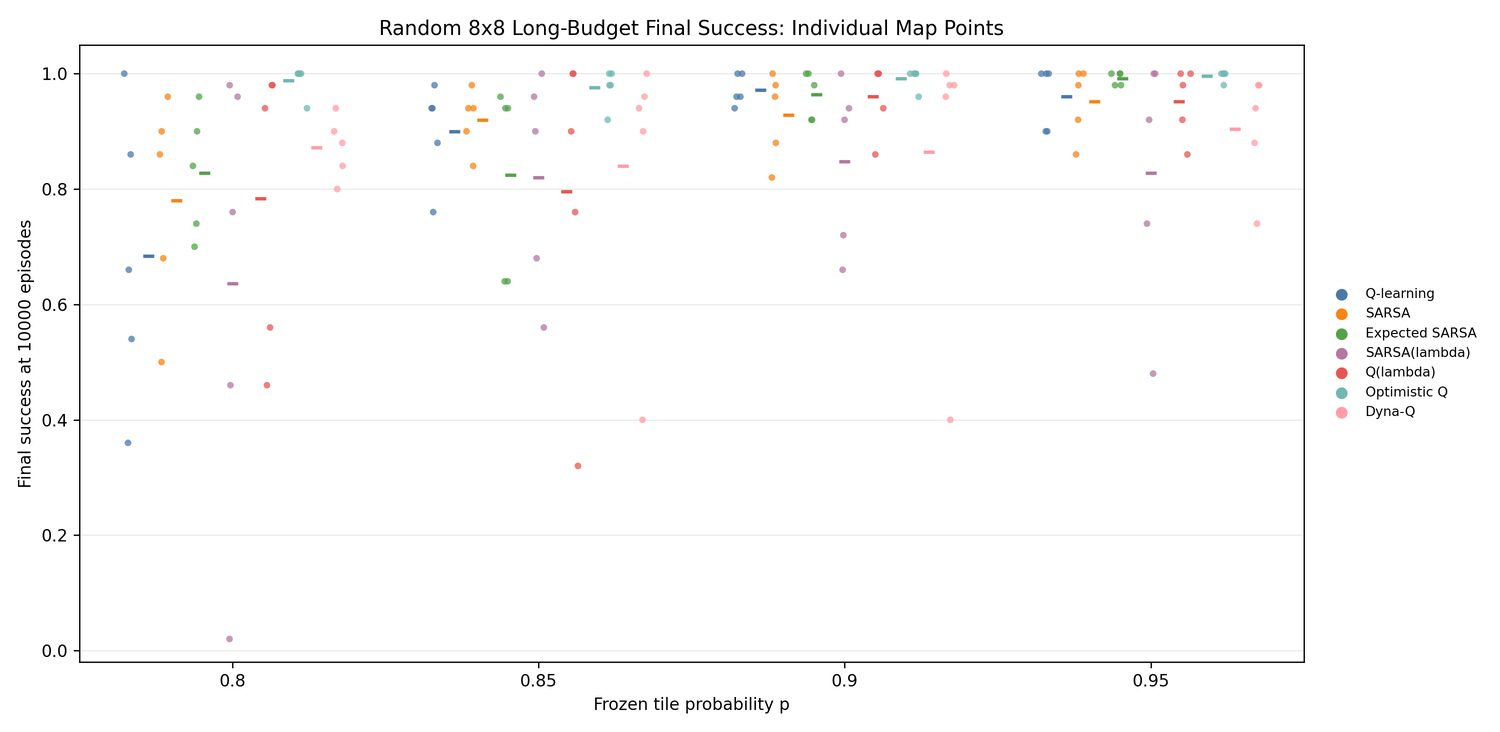
\includegraphics[width=0.9\linewidth]{figures_compact/random8_final_success_points_by_probability.jpg}
    \caption{Random 8$\times$8 slippery final success by frozen-tile probability after 10,000 training episodes. Each dot is one map.}
    \label{fig:difficulty}
\end{figure}

Figure~\ref{fig:learningpanel} shows per-map learning curves rather than one mixed curve. This directly addresses the variance problem: different maps have different learning difficulty even when their oracle success is high. The per-map plots show when an algorithm genuinely fails to converge on a specific layout.

\begin{figure}[H]
    \centering
    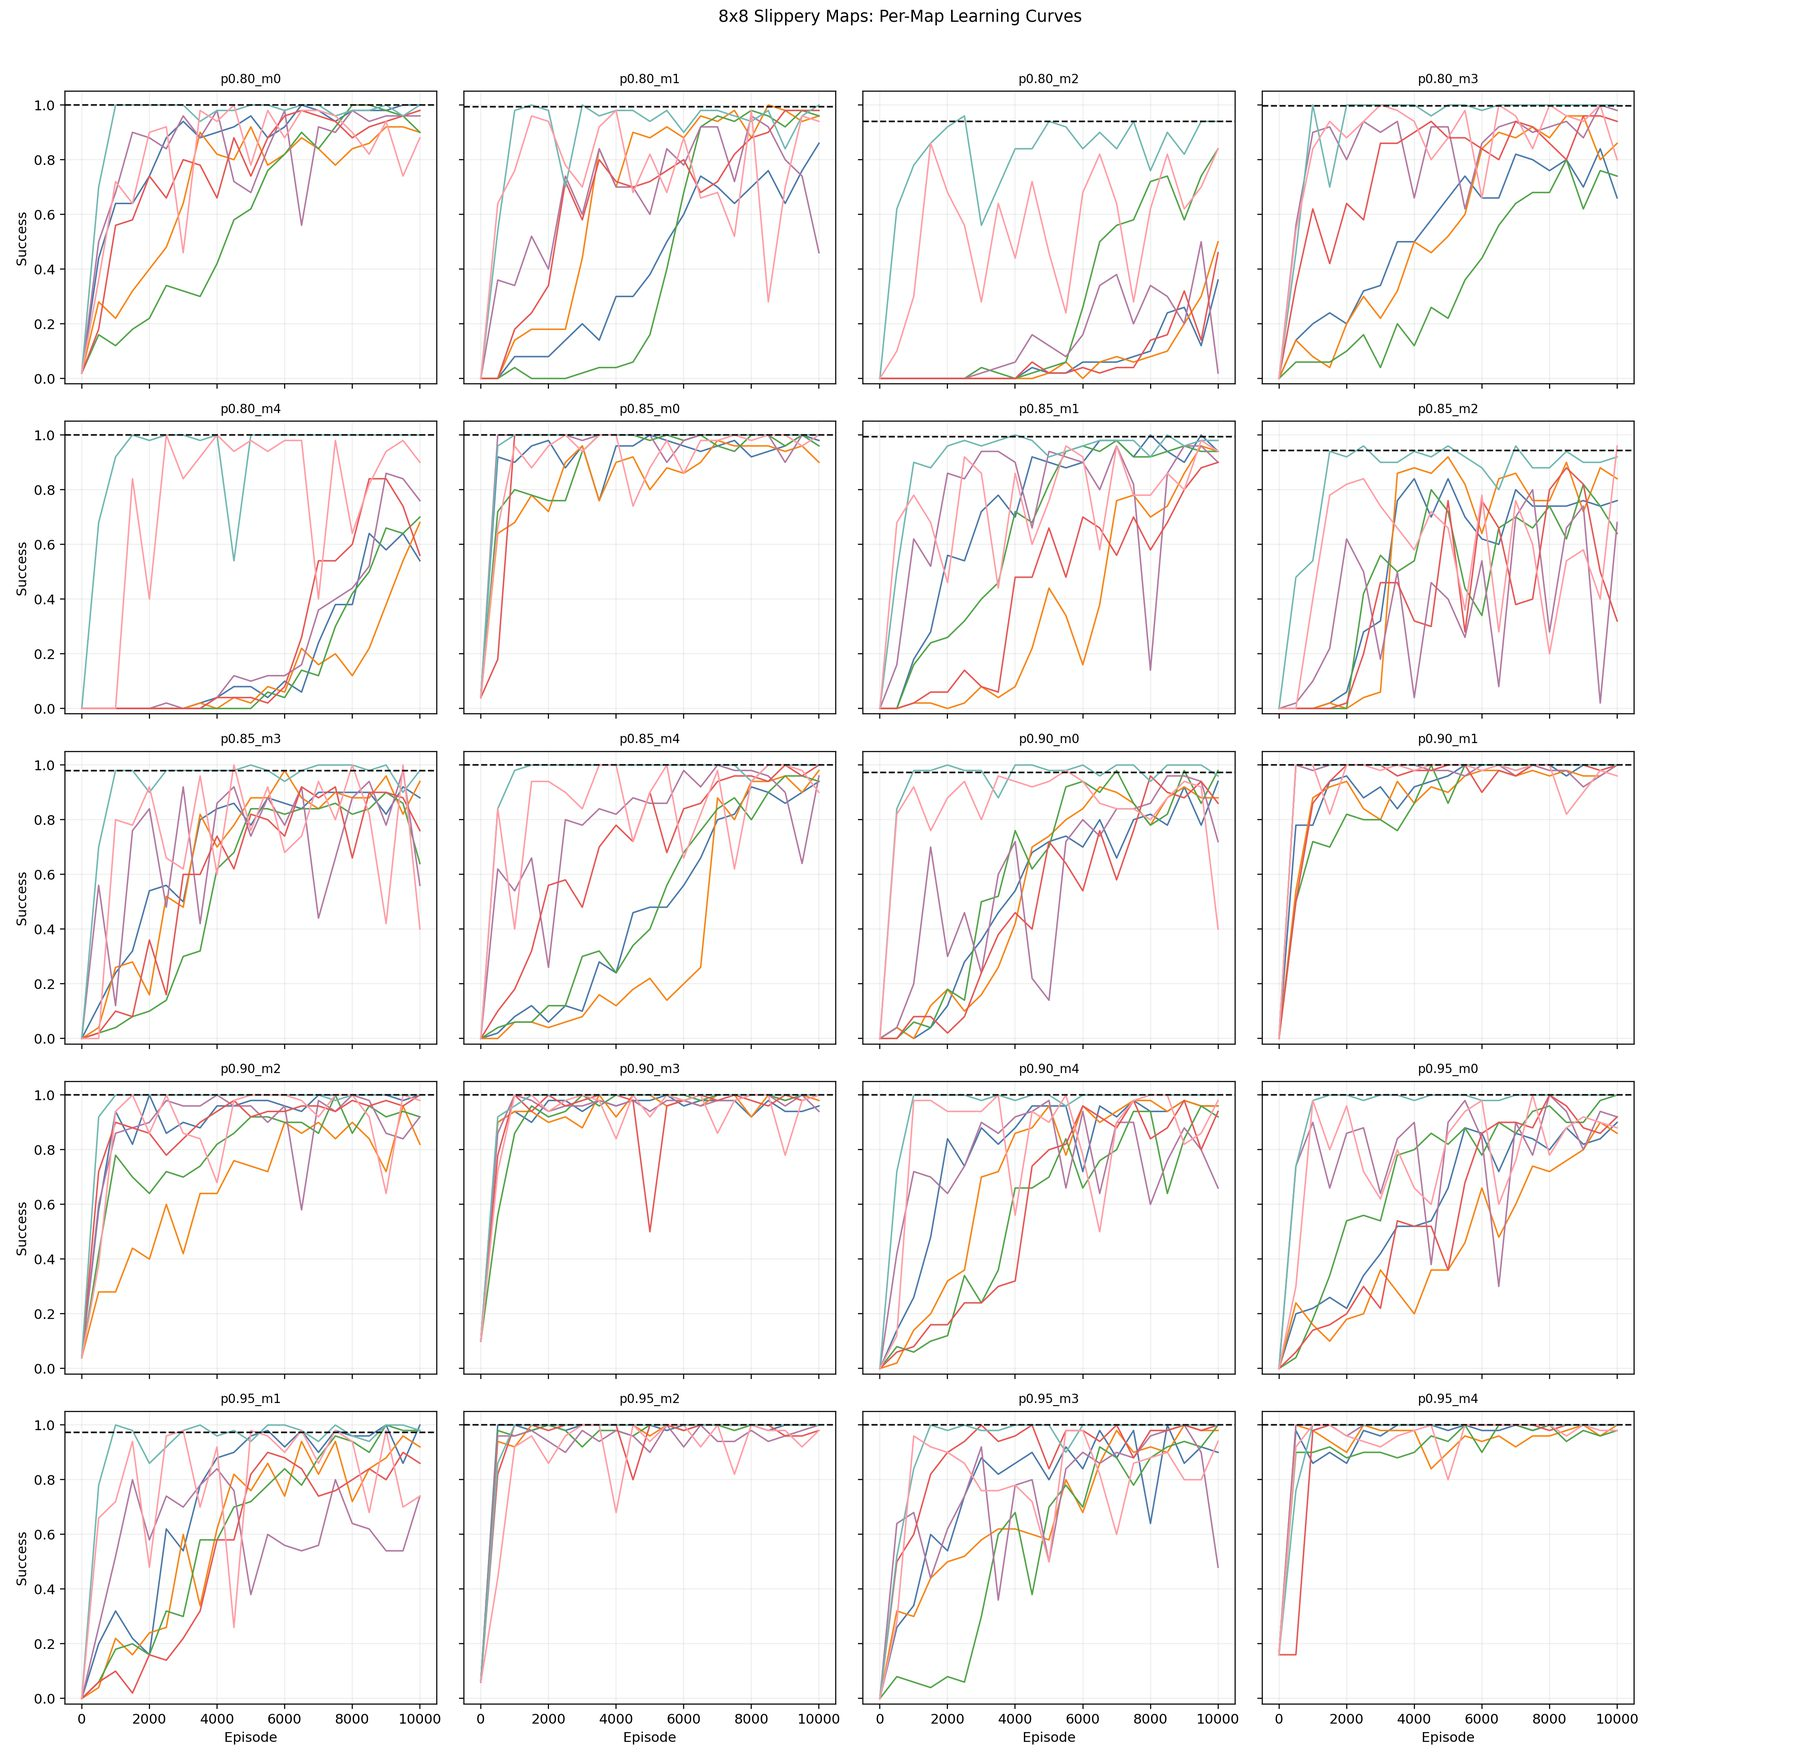
\includegraphics[width=0.96\linewidth]{figures_compact/random8_learning_curves_all_maps_panel.jpg}
    \caption{Per-map learning curves for 20 random 8$\times$8 slippery maps. Each subplot contains all seven algorithms and the Value Iteration oracle.}
    \label{fig:learningpanel}
\end{figure}

\subsection{Key Numerical Results}
Table~\ref{tab:keyresults} reports the latest stochastic-only results used in the analysis. The controlled random 8$\times$8 rows are the main random-map algorithm comparison; the Gymnasium rows are included separately as diagnostic evidence for why controlled maps were introduced.

\begin{table}[H]
\centering
\caption{Selected latest stochastic results. Success values are mean final greedy evaluation rates.}
\label{tab:keyresults}
\begin{tabular}{llcc}
\toprule
Setting & Method & Mean Success & Std. Dev.\\
\midrule
Standard 4$\times$4 & Value Iteration oracle & 0.847 & --\\
Standard 4$\times$4 & Q-learning & 0.770 & 0.046\\
Standard 4$\times$4 & Optimistic Q-learning & 0.767 & 0.025\\
Standard 4$\times$4 & SARSA & 0.723 & 0.021\\
\midrule
Designed 4$\times$4 & Value Iteration oracle & 0.708 & --\\
Designed 4$\times$4 & Expected SARSA & 0.635 & 0.199\\
Designed 4$\times$4 & Q-learning & 0.630 & 0.234\\
Designed 4$\times$4 & Optimistic Q-learning & 0.590 & 0.308\\
\midrule
Fixed 8$\times$8 & Optimistic Q-learning & 0.817 & 0.155\\
Fixed 8$\times$8 & Q-learning & 0.760 & 0.046\\
Fixed 8$\times$8 & Q($\lambda$) & 0.580 & 0.053\\
\midrule
Random 8$\times$8 & Value Iteration oracle & 0.988 & --\\
Random 8$\times$8 & Optimistic Q-learning & 0.988 & 0.023\\
Random 8$\times$8 & Expected SARSA & 0.902 & 0.122\\
Random 8$\times$8 & SARSA & 0.895 & 0.122\\
\midrule
Gymnasium standard 8$\times$8 & Expected SARSA & 0.850 & --\\
Gymnasium standard 8$\times$8 & Q($\lambda$) & 0.850 & --\\
Gymnasium standard 8$\times$8 & Optimistic Q-learning & 0.820 & --\\
Gymnasium all 8$\times$8 maps & Optimistic Q-learning & 0.235 & 0.327\\
Gymnasium all 8$\times$8 maps & SARSA($\lambda$) & 0.143 & 0.317\\
\bottomrule
\end{tabular}
\end{table}

\section{Ablation Study}
\subsection{Exploration Ablation}
Figure~\ref{fig:explore} isolates exploration strategy on fixed 8$\times$8 slippery FrozenLake. Optimistic Q-learning reaches 0.817 and Q-learning reaches 0.760. UCB-Q and softmax Q-learning perform poorly under this training budget, reaching 0.133 and 0.100. The result suggests that simple optimistic initialization is especially effective in this sparse tabular task: unknown actions remain attractive long enough for the agent to discover the goal.

\begin{figure}[H]
    \centering
    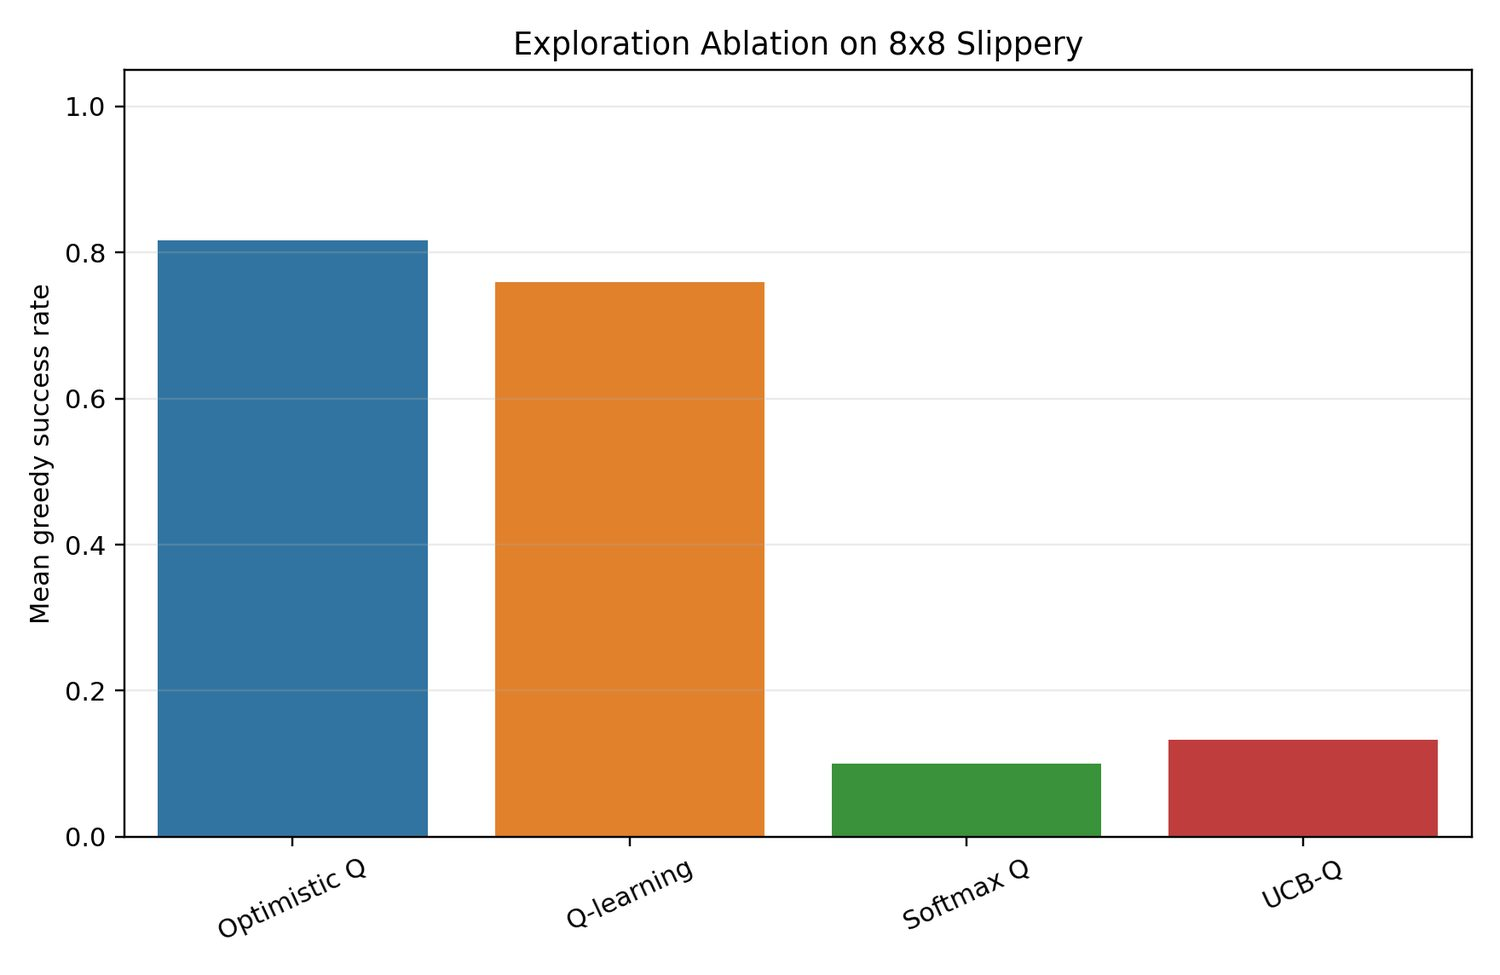
\includegraphics[width=0.76\linewidth]{figures_compact/exploration_ablation_fixed_8x8.jpg}
    \caption{Exploration ablation on fixed 8$\times$8 slippery FrozenLake. Optimistic initialization is the strongest exploration mechanism here.}
    \label{fig:explore}
\end{figure}

\subsection{Reward Propagation Ablation}
Figure~\ref{fig:propagation} compares methods that propagate sparse terminal reward in different ways. Q-learning is strongest on the fixed 8$\times$8 map at 0.760. Q($\lambda$), Dyna-Q, and SARSA($\lambda$) are lower on this fixed map but remain important because they improve robustness on random 8$\times$8 maps. n-step SARSA and Expected SARSA are highly variable, which is expected when successful episodes are rare and the behavior policy is still exploratory.

\begin{figure}[H]
    \centering
    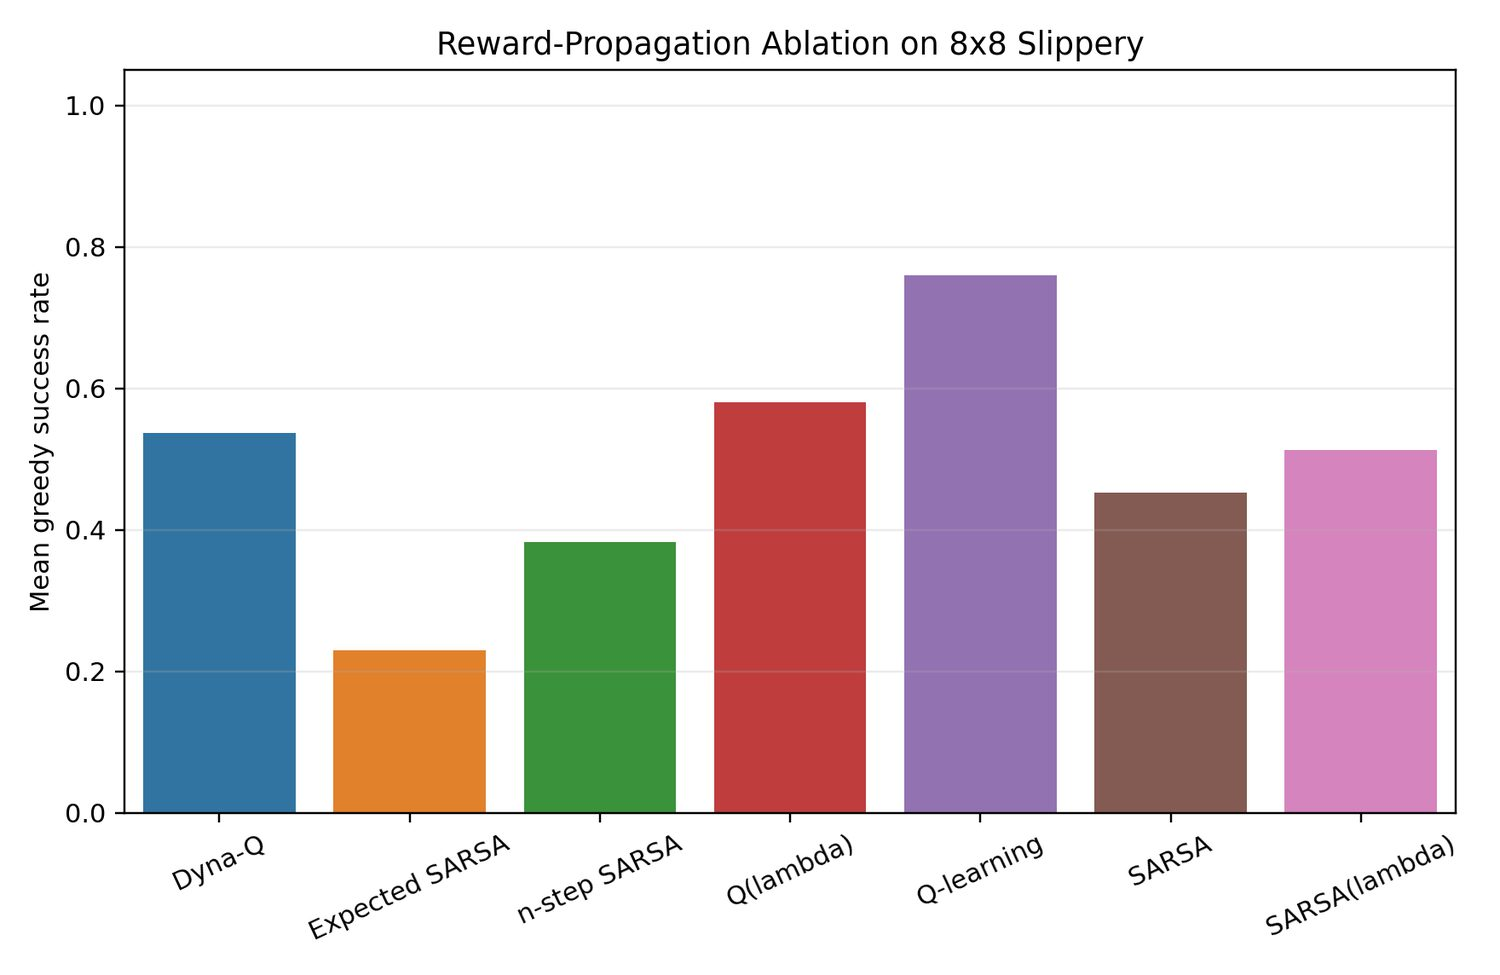
\includegraphics[width=0.78\linewidth]{figures_compact/reward_propagation_ablation_fixed_8x8.jpg}
    \caption{Reward-propagation ablation on fixed 8$\times$8 slippery FrozenLake. More complex propagation is not automatically better under short sparse-reward training.}
    \label{fig:propagation}
\end{figure}

\subsection{Oracle-Gap Ablation}
Figure~\ref{fig:gap} measures how far learned policies are from the known-model oracle on each random 8$\times$8 map. Optimistic Q-learning has the smallest mean gap after the long run. Some non-optimistic methods still have isolated hard-map failures, which is why per-map heatmaps are more useful than a single averaged line.

\begin{figure}[H]
    \centering
    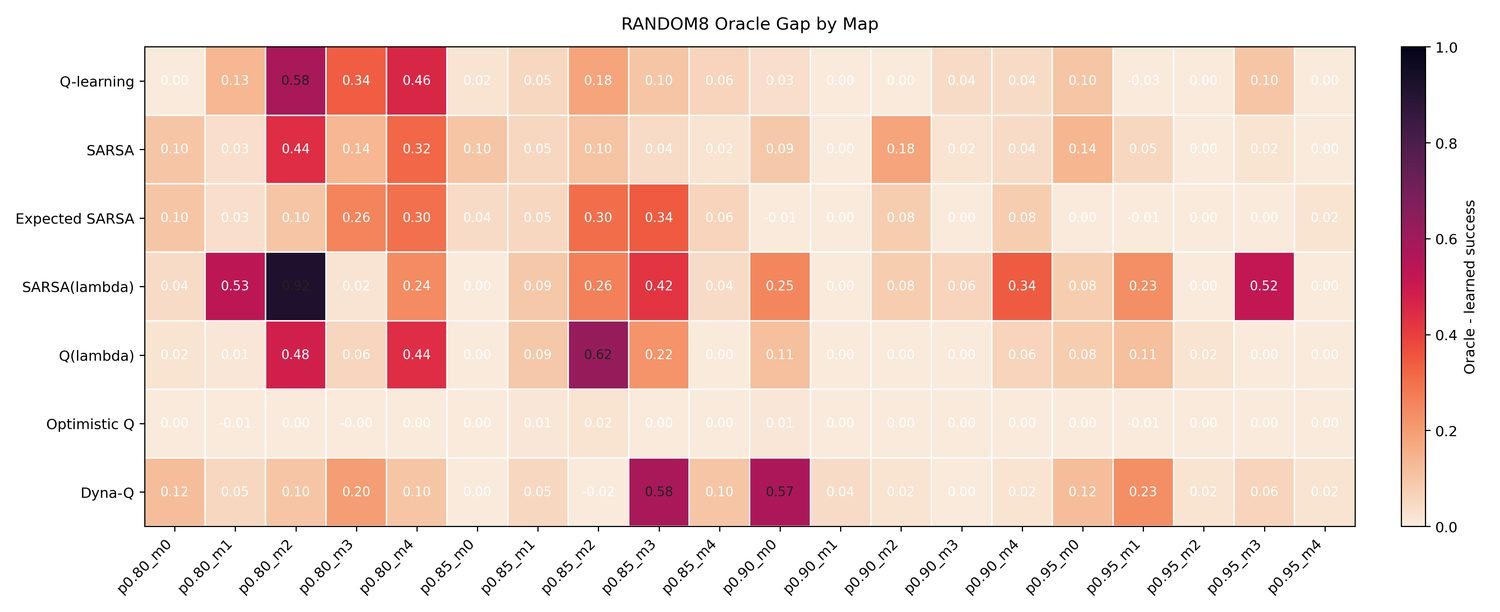
\includegraphics[width=0.96\linewidth]{figures_compact/random8_oracle_gap_heatmap_by_map.jpg}
    \caption{Oracle gap on random 8$\times$8 slippery maps after 10,000 training episodes. Lower is better. Every cell is explicitly annotated.}
    \label{fig:gap}
\end{figure}

Figure~\ref{fig:aucconv} gives two additional views: AUC measures how good the whole learning process is, while the convergence heatmap reports the first episode at which success reaches 0.80. Dyna-Q has a high mean AUC and early average convergence, even though its final score is slightly below the strongest methods.

\begin{figure}[H]
    \centering
    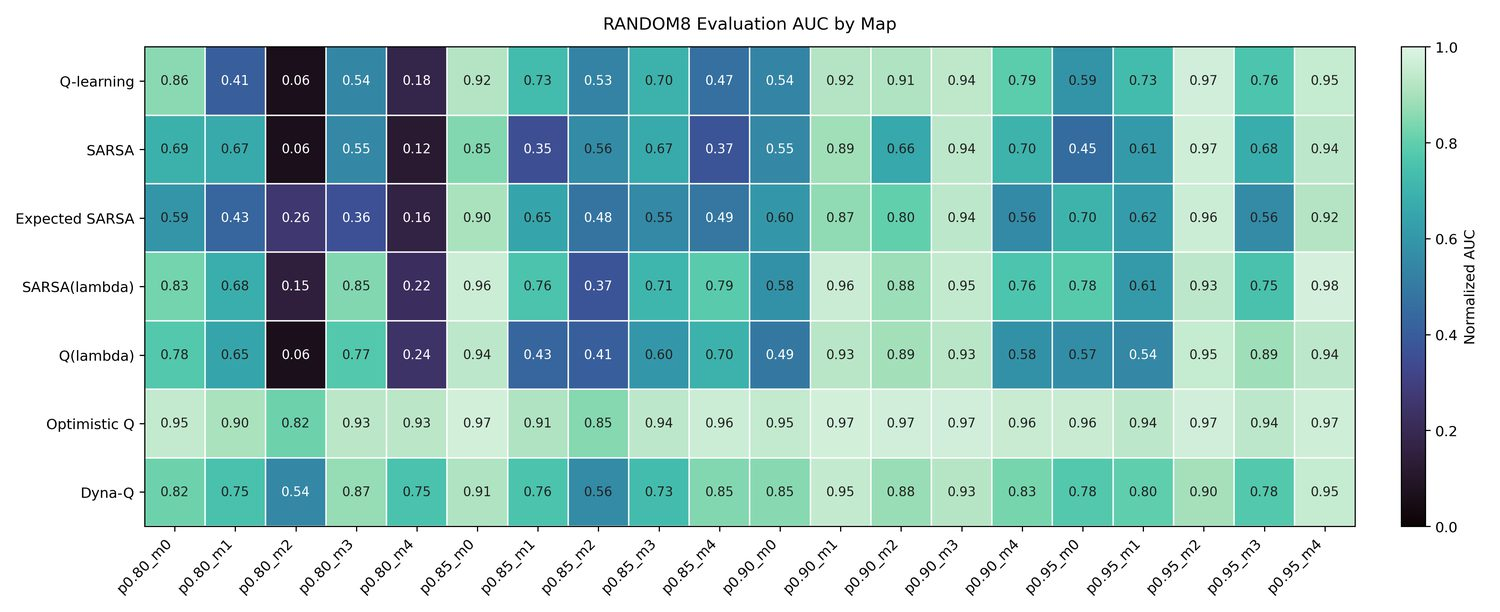
\includegraphics[width=0.96\linewidth]{figures_compact/random8_auc_heatmap_by_map.jpg}
    \caption{Evaluation AUC by algorithm and random 8$\times$8 map. Higher values mean better performance throughout training, not only at the end.}
    \label{fig:aucconv}
\end{figure}

\section{Hyperparameter Optimization}
We use Optuna with the TPE sampler because it is simple to run locally, supports conditional search spaces, and is sufficient for the size of this project. A key lesson is that the search space must match the algorithm. A generic search over learning rate, discount factor, and epsilon schedule is incomplete for methods like optimistic Q-learning and Dyna-Q. After adding \texttt{optimistic\_init} and \texttt{planning\_steps}, tuning became more meaningful.

On fixed 8$\times$8 stochastic FrozenLake, the best Optuna validation scores were 0.830 for optimistic Q-learning, 0.795 for Dyna-Q, 0.735 for Q-learning, and 0.665 for Expected SARSA. Three-seed validation confirmed tuned optimistic Q-learning and tuned Dyna-Q as the strongest tuned candidates. Optuna is therefore a good choice for this report; Ray Tune would be more appropriate only if we scaled to many more maps or GPU-based neural RL.

\begin{figure}[H]
    \centering
    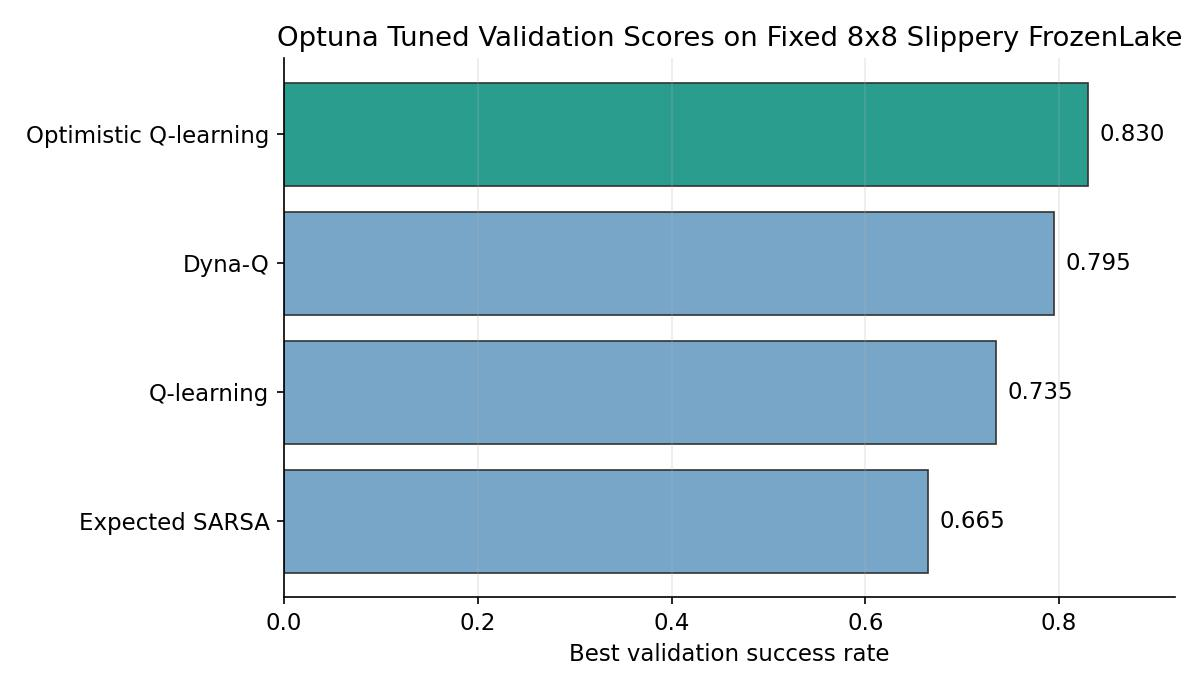
\includegraphics[width=0.72\linewidth]{figures_compact/optuna_best_scores.jpg}
    \caption{Best Optuna validation scores on fixed 8$\times$8 stochastic FrozenLake.}
    \label{fig:optuna}
\end{figure}

\section{Discussion}
The results show that map design is not a minor implementation detail; it determines whether FrozenLake is a meaningful comparison task. The Gymnasium standard 8$\times$8 board confirms that the training pipeline can solve a recognized stochastic benchmark, while the Gymnasium random-map diagnostic shows that deterministic reachability alone is insufficient under slippery transitions. Once the benchmark is controlled so that maps are solvable, non-trivial, and reproducible, the algorithm differences become much easier to interpret.

On the controlled 8$\times$8 benchmark, exploration matters more than raw algorithmic complexity. Optimistic Q-learning performs best because optimistic initial values actively encourage the agent to try uncertain actions, which is crucial when the only positive reward is at the goal. The long-budget results also clarify an earlier concern: the large standard deviations in short-budget random-map plots mainly came from mixing maps with different layouts before the algorithms had enough time to converge. When each map is plotted separately and the 8$\times$8 budget is increased to 10,000 episodes, most tabular methods improve greatly on the controlled maps.

Dyna-Q and eligibility traces answer a different problem: once reward is found, how quickly can it be reused or propagated backward? In the final-success ranking, Dyna-Q is not the best long-budget method, but its AUC and convergence behavior are strong. This means Dyna-Q is valuable when sample efficiency during training matters, while optimistic Q-learning remains the strongest final-policy choice.

The board design results are important. A single fixed board is reproducible but not enough for validation, but some fixed boards are still essential standards. The Gymnasium standard 8$\times$8 board is one such case: it is a useful common reference and confirms that our agents can learn a recognized stochastic game benchmark. Random boards are also valuable, but their role must be stated clearly. Our workflow reflects this: the Gymnasium random-map attempt exposed many near-zero oracle boards, so we moved to controlled boards for the main comparison. For 4$\times$4, boards need a controlled hole count, reachability checks, and oracle filtering; otherwise the game can accidentally become too easy. For 8$\times$8, the controlled random boards are appropriate for comparing agents because they produce solvable stochastic tasks with meaningful variation. The Gymnasium random-map diagnostic remains valuable because it explains the boundary of the claim: lower-$p$ random boards may be connected in the deterministic sense but nearly impossible under slippery transitions.

We intentionally exclude exploratory neural-RL stress tests from the final benchmark because their current results were not competitive on this sparse tabular task under the available budget. Including them would distract from the validated stochastic tabular comparison. Similarly, 16$\times$16 maps are kept as future work because current results depend strongly on special map design, reward shaping, or much larger training budgets.

\section{Conclusion}
We converted the original 4$\times$4 Q-learning game-playing project into a broader stochastic FrozenLake study with multiple tabular agents, controlled random boards, Value Iteration oracle references, Optuna tuning, ablation studies, and long-budget per-map learning curves. The key methodological contribution is the board-design refinement: the Gymnasium standard 8$\times$8 board provides an important standard game comparison, but direct Gymnasium random boards were too often near-impossible under slippery dynamics, so controlled boards were introduced to make agent comparison meaningful. The central algorithmic result is that optimistic Q-learning is the strongest learned game-playing agent on the controlled stochastic benchmark, achieving near-oracle performance on controlled random 8$\times$8 boards. Expected SARSA, SARSA, and Q-learning form a strong second group, while Dyna-Q is more attractive when learning speed and AUC matter. The final practical recommendation is therefore: use Q-learning as a baseline agent, add optimistic exploration, validate on standard boards such as Gymnasium 8$\times$8, compare algorithms on controlled stochastic boards, and use Gymnasium-generated boards plus oracle gaps as a diagnostic check before making broad claims about random-map generalization.

\bibliographystyle{IEEEtran}
\bibliography{references}

\end{document}
